\documentclass[11pt,a4paper]{jsarticle}
%
\usepackage{amsmath,amssymb}
\usepackage{bm}
\usepackage{graphicx}
\usepackage{ascmac}
\usepackage{amsmath}
\usepackage{amsfonts}
\usepackage{amsthm}
\usepackage{amssymb}
\usepackage{bm}
\usepackage{mathtools}
% 画像
%
\setlength{\textwidth}{\fullwidth}
\setlength{\textheight}{39\baselineskip}
\addtolength{\textheight}{\topskip}
\setlength{\voffset}{-0.5in}
\setlength{\headsep}{0.3in}

\newtheorem{thm}{Theorem}[section]
\newtheorem{prop}[thm]{Proposition}
\newtheorem{lem}[thm]{Lemma}
\newtheorem{cor}[thm]{Corollary}
\newtheorem{conj}[thm]{Conjecture}
\theoremstyle{definition}
\newtheorem{dfn}[thm]{Definition}
\newtheorem{rem}[thm]{Remark}
\newtheorem{fact}[thm]{Fact}

\newcommand{\RealNumberSet}{\mathbb{R}}

%
\pagestyle{myheadings}
\begin{document}
%
%
\section{連結性と弧状連結性}

\begin{dfn}{(位相空間の連結性)}
  位相空間 $(X, \mathcal{O})$ が連結であるとは、$X$ の部分集合であって、
  $(X, \mathcal{O})$ の開集合かつ閉集合であるものが、空集合 $\emptyset$ と
  全空間 $X$ のみであることをいう。
\end{dfn}

\begin{lem}
  位相空間 $(X, \mathcal{O})$ が連結であることと、以下の性質が成り立つことは同値である。
  もし $U, V \in \mathcal{O}$ が空でない開集合であり、$X = U \cup V$ ならば、 
  $U \cap V \ne \emptyset$
\end{lem}

\begin{proof}
  待遇を示す。$U \in X$ を空でない、全空間と等しくない部分集合とし、この集合は開集合かつ閉集合であると仮定する。
  このとき、$ V = X \backslash U$ とすると、$U$ と $V$ はどちらも開集合となり、
  $X = U \cup V$、$U \cap V = \emptyset$ となる。逆を示す。
  $X = U \cup V$ と $U \cap V = \emptyset$ を満たす $X$ の空でない、
  また全空間と等しくない開集合 $U, V$ について、$U = X \backslash V$ が成り立つ。
  したがって、$U$ は開集合かつ閉集合となる。
\end{proof}

\begin{dfn}
  $(X, \mathcal{O})$ を位相空間とする。$X$ の空でない部分集合 $A$ に対して、
  \begin{equation}
    \mathcal{O}_{A} = \{ U \cap A \:|\: U \in \mathcal{O} \} \notag
  \end{equation}
  と定めると、$\mathcal{O}_{A}$ は $A$ の一つの位相である。この位相 $\mathcal{O}_{A}$ を集合 $A$
  上の $\mathcal{O}$ に関する相対位相という、また、位相空間 $(A, \mathcal{O}_{A})$ を、
  位相空間 $(X, \mathcal{O})$ の部分空間という。
\end{dfn}

\begin{rem}
  $(X, \mathcal{O})$ を位相空間、$A$ を $(X, \mathcal{O})$ の部分集合とする。
  Lemma~1.2 を用いることで、集合 $A$ が連結であることの定義は、以下の性質を満たすことである。
  もし $U, V $ が $X$ の開集合であり、$A \cap U \ne \emptyset$ と
  $A \cap V \ne \emptyset$ を満たし、$A \subset U \cup V$ ならば、
  $A \cap U \cap V \ne \emptyset$ が成り立つ。
\end{rem}

\begin{figure}[h]
  \centering
  \begin{minipage}[b]{0.49\columnwidth}
      \centering
      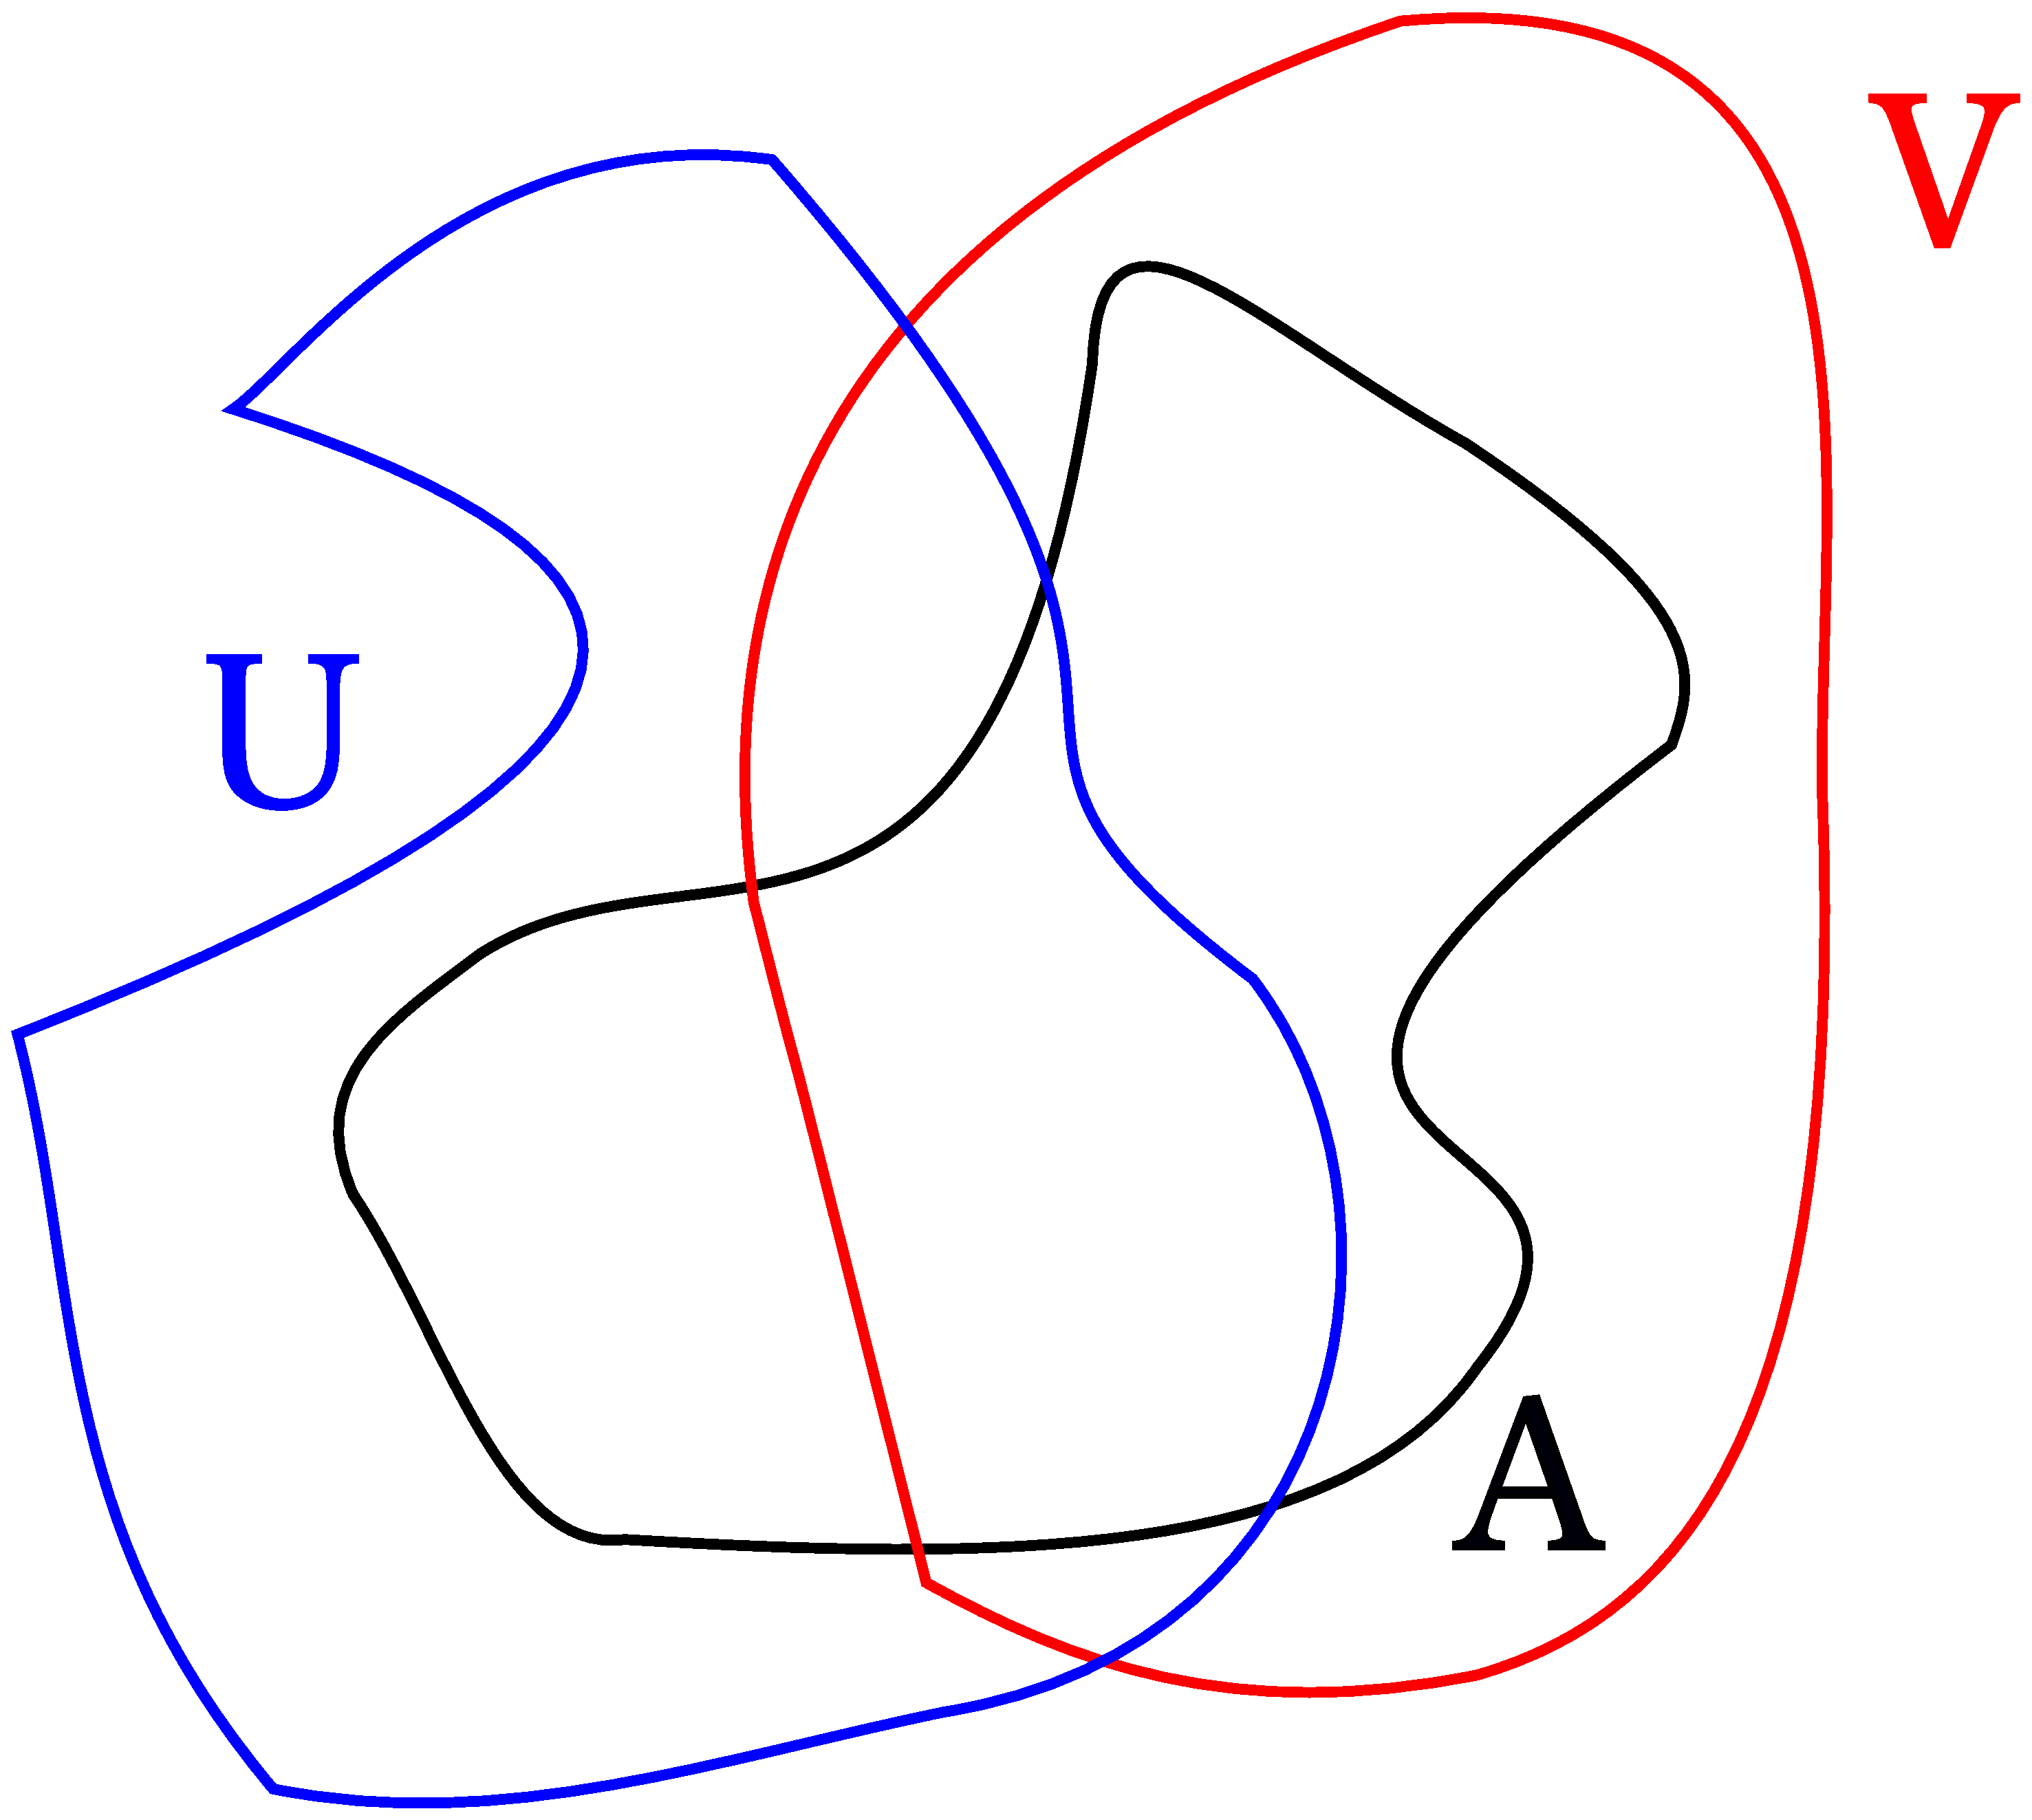
\includegraphics[width=0.7\columnwidth]{figures/eps/connected.eps}
      \caption{Aが連結集合であるとき}
      \label{fig:a}
  \end{minipage}
  \begin{minipage}[b]{0.49\columnwidth}
      \centering
      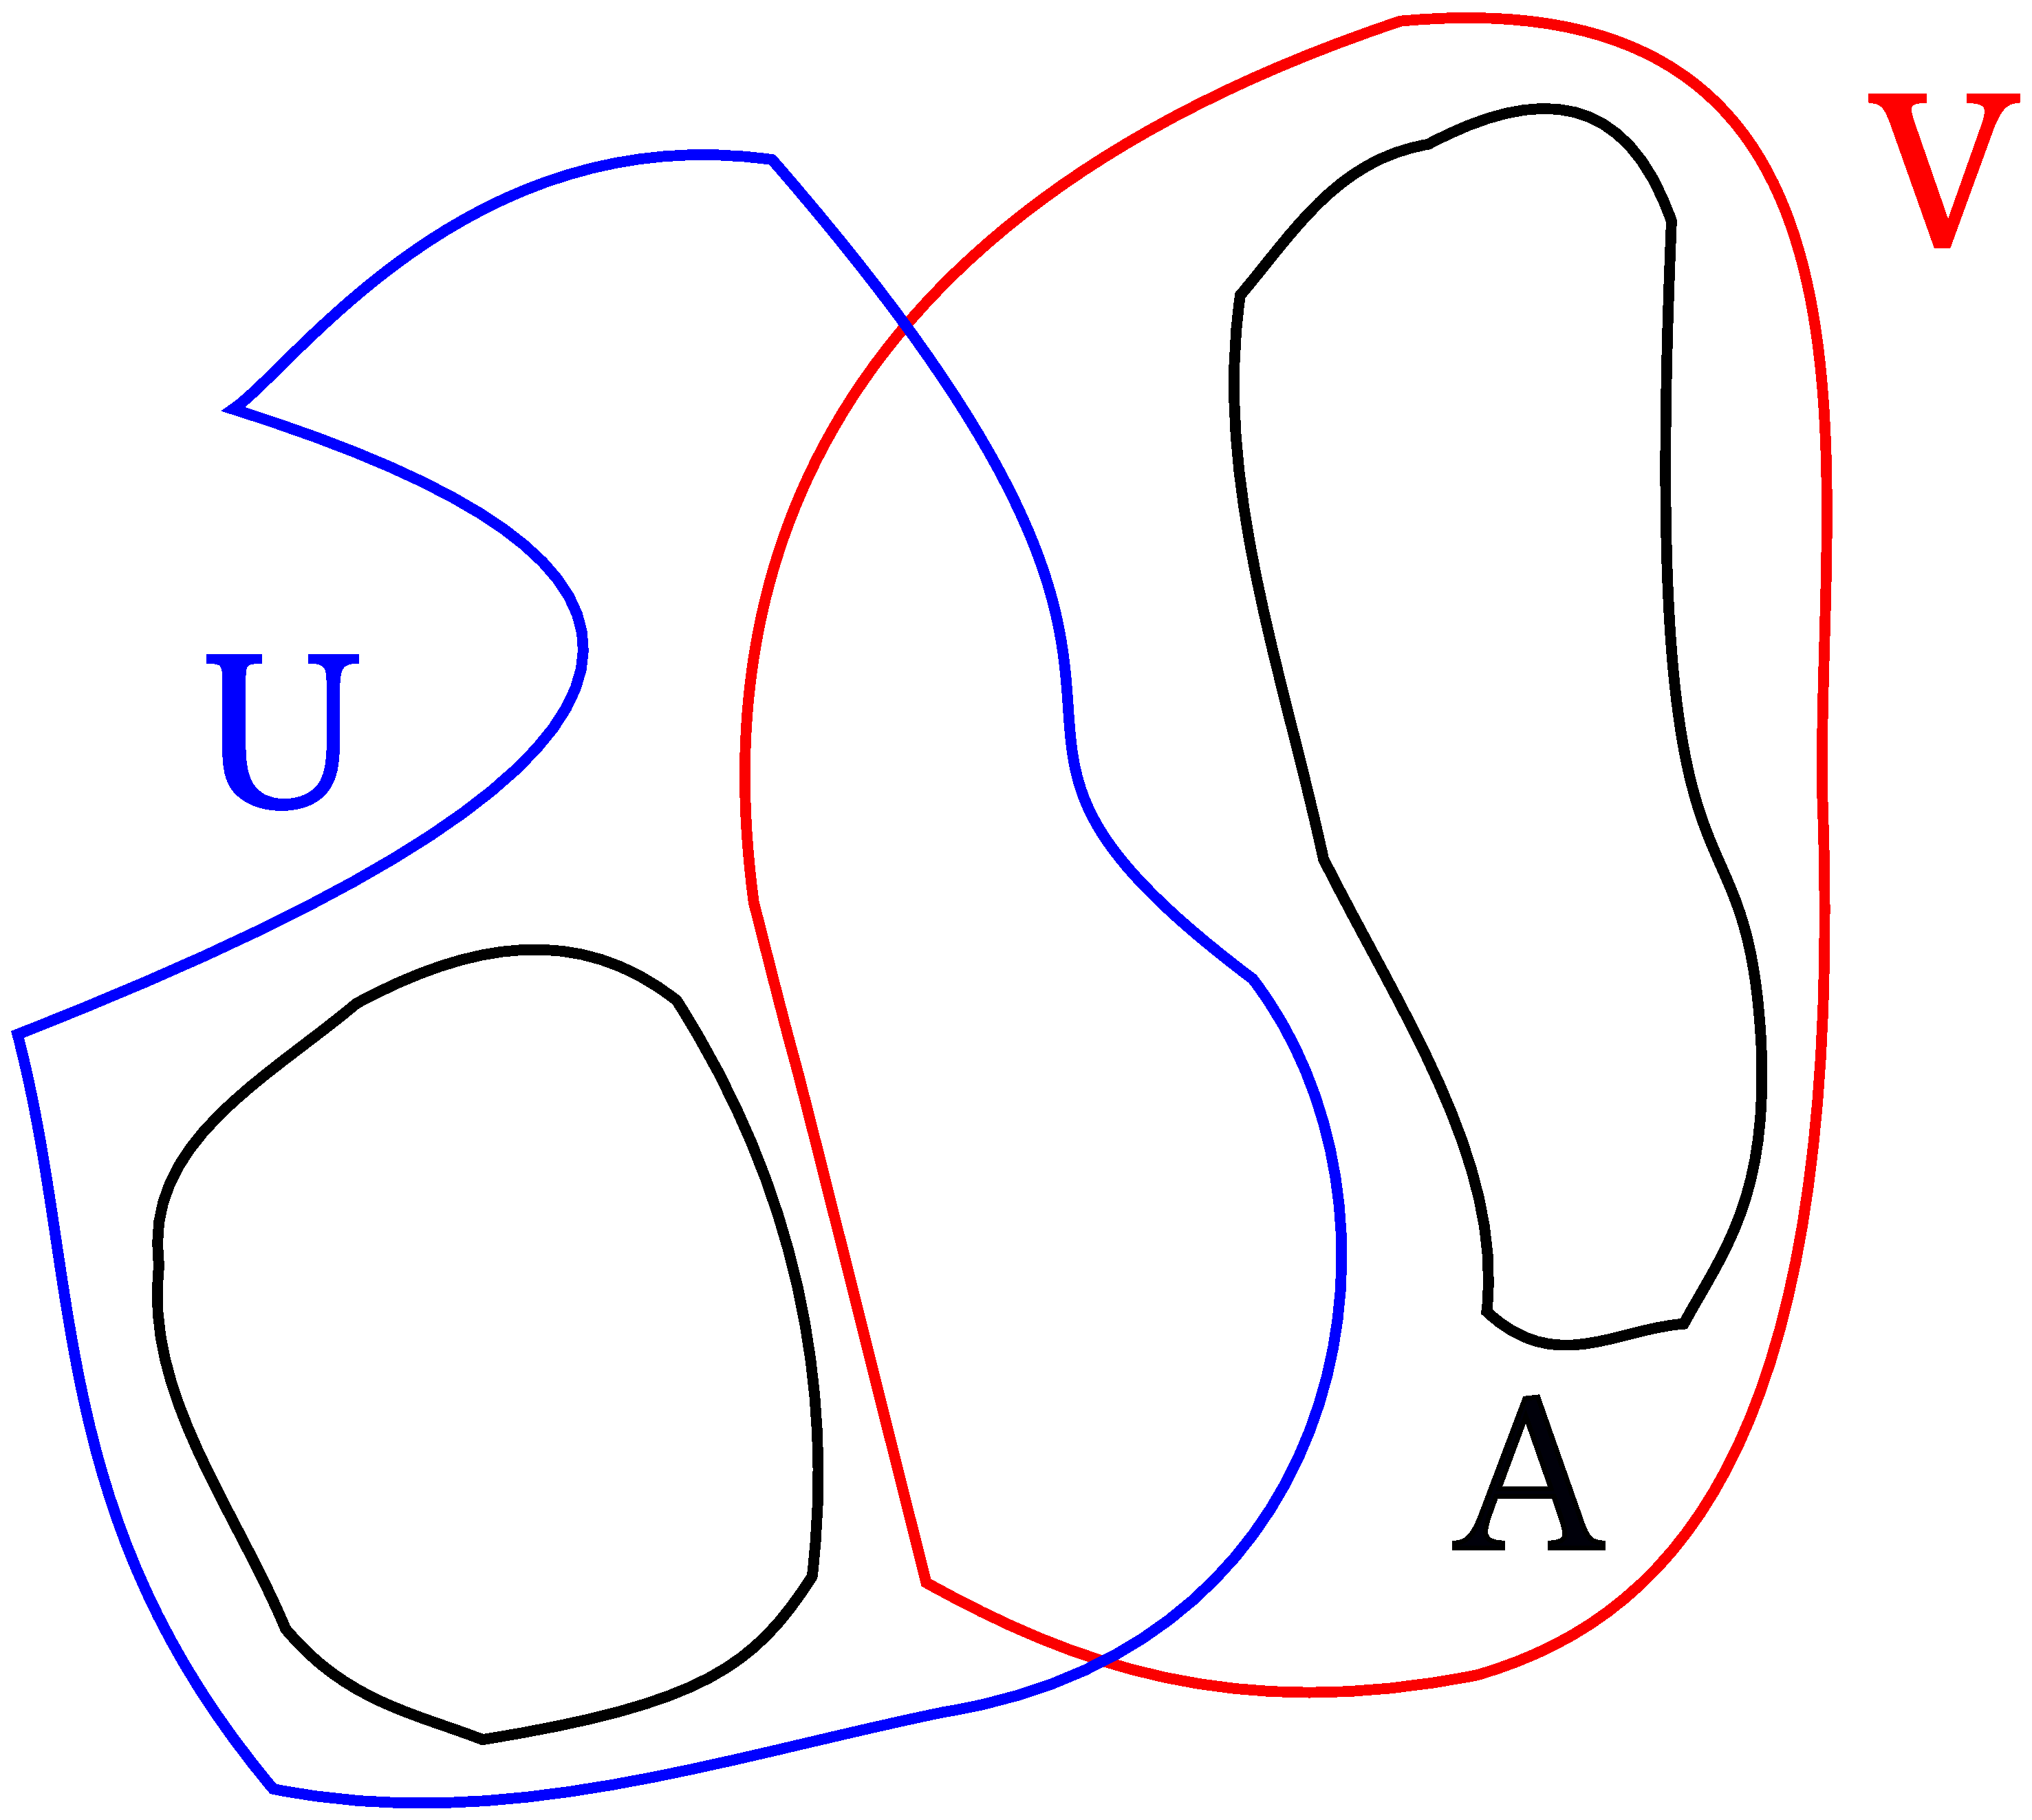
\includegraphics[width=0.7\columnwidth]{figures/eps/not_connected.eps}
      \caption{Aが連結集合でないとき}
      \label{fig:b}
  \end{minipage}
  \end{figure}

\begin{dfn}
  位相空間 $X$ が弧状連結であるとは、任意の $x_{0}, x_{1} \in X$ に対して、
  ある連続写像 $f: [0, 1] \to X$ が存在して、$f(0) = x_{0}$ かつ $f(1) = x_{1}$
  が成り立つことをいう。$[0,1]$ には $\RealNumberSet$ の部分集合としての通常の位相が入っているものとする。
  $f$ あるいは $f$ の像 $f([0, 1])$ をパスと呼ぶ。
\end{dfn}
%
%
\end{document}